\hypertarget{a00001_lang}{}\section{Language}\label{a00001_lang}
For remote programmming operations the burn in unit uses commands that follow the S\-C\-P\-I syntax as outlined in the System for Standard Commands for Programmable Instruments for C28x Code Reference Manual, where in the standard programmming commands that are included by this system are also outlined. Please refer to that document and, where necessray, any further referenced documents, for inforrmation on the syntax of the programming commands.

This unit programming chapter will focus on the function of the commands specific to the burn in unit\hypertarget{a00001_format}{}\subsection{Format}\label{a00001_format}
The burn in unit uses a standard raw T\-C\-P/\-I\-P Ethernet connection to communicate with a controlling system. Once the user's control system has established a valid raw T\-C\-P/\-I\-P connection with the burn in unit commands should be sent and received as A\-S\-C\-I\-I character byte string data, with the most significant byte first.

Thus the data sent that would correspond to the {\ttfamily $<$}C\-O\-M\-M\-O\-N Q\-U\-E\-R\-Y P\-R\-O\-G\-R\-A\-M H\-E\-A\-D\-E\-R{\ttfamily $>$} {\ttfamily $\ast$\-I\-D\-N}?; in transmission order would be (including the '$^\wedge$\-N\-L' {\ttfamily $<$}P\-R\-O\-G\-R\-A\-M M\-E\-S\-S\-A\-G\-E T\-E\-R\-M\-I\-N\-A\-T\-O\-R{\ttfamily $>$}) \begin{quotation}
{\ttfamily 0x2\-A 0x49 0x44 0x4\-E 0x3\-F 0x3\-B 0x0\-A}

\end{quotation}
\hypertarget{a00001_progcreation}{}\subsection{Program Message Unit Creation}\label{a00001_progcreation}
The user may create a {\ttfamily $<$}P\-R\-O\-G\-R\-A\-M M\-E\-S\-S\-A\-G\-E U\-N\-I\-T{\ttfamily $>$} by traversing the command tree from the root towards the desired function and concatenating the {\ttfamily $<$}program mnemonic{\ttfamily $>$}s and {\ttfamily $<$}C\-O\-M\-M\-A\-N\-D P\-R\-O\-G\-R\-A\-M H\-E\-A\-D\-E\-R{\ttfamily $>$} or {\ttfamily $<$}Q\-U\-E\-R\-Y P\-R\-O\-G\-R\-A\-M H\-E\-A\-D\-E\-R{\ttfamily $>$} stepped through to reach that destination.

For example, using the hypothetical command tree shown in the following figure, the {\ttfamily $<$}P\-R\-O\-G\-R\-A\-M M\-E\-S\-S\-A\-G\-E U\-N\-I\-T{\ttfamily $>$} required to run the function 'E\-E\-E' would be\-: \begin{quotation}
{\ttfamily B\-B\-B\-:E\-E\-E;}

\end{quotation}


\begin{center}

\begin{DoxyImageNoCaption}
  \mbox{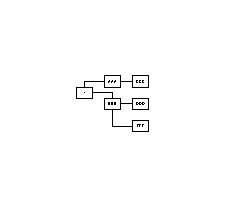
\includegraphics[width=\textwidth,height=\textheight/2,keepaspectratio=true]{dot_inline_dotgraph_1}}
\end{DoxyImageNoCaption}
\end{center}
\hypertarget{a00001_queries}{}\subsection{Queries and Responses}\label{a00001_queries}
Each {\ttfamily $<$}P\-R\-O\-G\-R\-A\-M M\-E\-S\-S\-A\-G\-E{\ttfamily $>$} may contain only one {\ttfamily $<$}Q\-U\-E\-R\-Y P\-R\-O\-G\-R\-A\-M H\-E\-A\-D\-E\-R{\ttfamily $>$} which, if used, should be the last header in the message. If a {\ttfamily $<$}Q\-U\-E\-R\-Y P\-R\-O\-G\-R\-A\-M H\-E\-A\-D\-E\-R{\ttfamily $>$} is used the next operation should be to read the response generated by the query, before any further {\ttfamily $<$}P\-R\-O\-G\-R\-A\-M M\-E\-S\-S\-A\-G\-E{\ttfamily $>$} elements are sent to the unit.\hypertarget{a00001_device}{}\section{Instrument Selection}\label{a00001_device}
Each burn in unit is split into several logical instruments that corresponds to the functional sections of the burn in unit. The instruement selection is controlled using the {\ttfamily I\-N\-S\-Trument} sub-\/system These instruments are numbered according to the unit channel numbering shown in the following list. These numbers can be obtained by using the {\ttfamily C\-A\-Talog}? query from the {\ttfamily I\-N\-S\-Trument} subsystem\-: \begin{quotation}
{\ttfamily I\-N\-S\-Trument\-:C\-A\-Talog?;}.

\end{quotation}


\begin{enumerate}\setcounter{enumi}{-1} \item Load 0 \item Load 1 \item Load 2 \item Load 3 \item AC Current Control \item DC Stage \item AC Stage \end{enumerate}

This means that before setting any of the instruments' settings, the relevant instrument number must first be selected. This is done using the {\ttfamily N\-S\-E\-Lect} command from the {\ttfamily I\-N\-S\-Trument} subsystem. The default instrument selection is 0. Once selected the value is \char`\"{}sticky\char`\"{}, and does not need to be set again until the user settings wishes to send commands for a different instrument. Thus, for example, the {\ttfamily $<$}P\-R\-O\-G\-R\-A\-M M\-E\-S\-S\-A\-G\-E{\ttfamily $>$} required to set the voltage level D\-C stage to 10 volts with a range set to 1\-V/\-V would be as follows\-: \begin{quotation}
{\ttfamily I\-N\-S\-Trument\-:N\-S\-E\-Lect 5;\-:S\-O\-U\-Rce\-:\-V\-O\-L\-Tage\-:L\-E\-Vel 10;\-:S\-O\-U\-Rce\-:\-V\-O\-L\-Tage\-:R\-A\-N\-Ge 1;}

\end{quotation}
\hypertarget{a00001_tree}{}\section{The Command Tree}\label{a00001_tree}
The command tree provides the structure of the subsystems and their commands. As shown however the diagram does not illustrate that some of the commands have no meaning to some instruments. For example, attempting to set the voltage coefficients of a current controlled instrument will result in an error.

Again, the commands shown here are in addition to those that are implemented as standard by the System for Standard Commands for Programmable Instruments for C28x.

The diagram is followed by a listing of each command. The next section, \hyperlink{a00002}{Command Reference} explains the operation and details of each command.

\begin{center}

\begin{DoxyImageNoCaption}
  \mbox{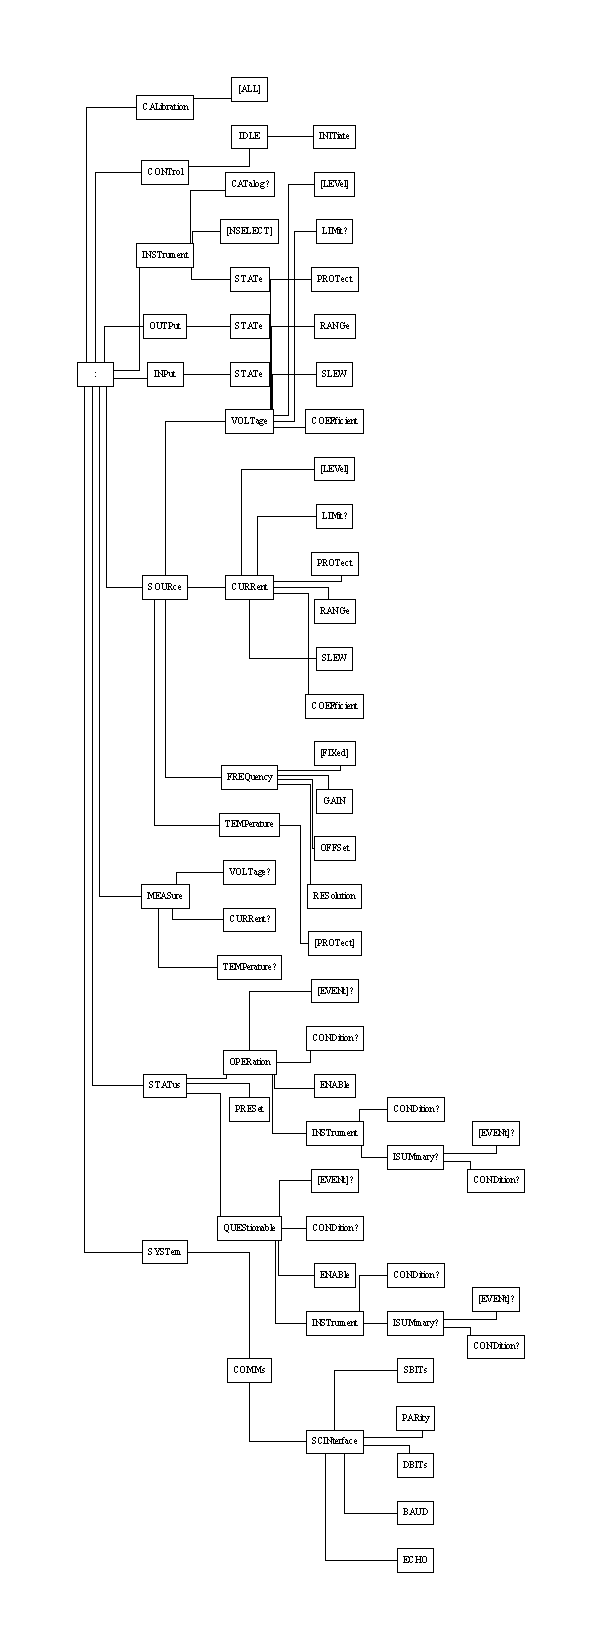
\includegraphics[width=\textwidth,height=\textheight/2,keepaspectratio=true]{dot_inline_dotgraph_2}}
\end{DoxyImageNoCaption}
\end{center}



\begin{DoxyPre}
{\bfseries CALibration}
    ALL
{\bfseries CONTrol}
    IDLE
        INITiate
{\bfseries INSTrument}
    CATalog?
    NSELect
    STATe
{\bfseries OUTPut}
    STATe
{\bfseries INPut}
    STATe
{\bfseries SOURce}
    VOLTage
        LEVel
        LIMit?
        PROTect
        RANGe
        SLEW
        COEFficient
    CURRent
        LEVel
        LIMit?
        PROTect
        RANGe
        SLEW
        COEFficient
    FREQuency
        FIXed
        GAIN
        OFFSet
    TEMPerature
        PROTect
{\bfseries MEASure}
    VOLTage?
    CURRent?
    TEMPerature?
{\bfseries STATus}
    OPERation
    PRESet
    QUEStionable
{\bfseries SYSTem}
    COMMs
        SCINterface
            SBITs
            PARity
            DBITs
            BAUD
            ECHO
\end{DoxyPre}
 